\documentclass[12pt, a4paper]{article}

\usepackage[utf8]{inputenc}
\usepackage{amsmath}
\usepackage{amsfonts}
\usepackage{amssymb}
\usepackage{graphicx}
\usepackage{booktabs}
\usepackage[margin=1in]{geometry}
\usepackage{setspace}
\usepackage{float}
\usepackage{parskip} % ADDED: Removes indents and adds space between paragraphs
\usepackage[round,authoryear]{natbib}
\usepackage[colorlinks=true, linkcolor=blue, citecolor=blue, urlcolor=blue]{hyperref}

\setstretch{1.15}

\title{\textbf{Replication and Extension of Strong Progenitor Age-Bias in Supernova Cosmology: Alignment with DESI BAO and Alternative Dark Energy Parametrizations}}

\author{
    Saravanan Sivaram Jeychand$^{1}$ \\
    Ng Shao Chin Cindy$^{1}$ \\
    \vspace{0.2cm} \\
    \small $^{1}$ \textit{Department of Physics, National University of Singapore} \\
    \small \textit{2 Science Drive 3, Singapore 117551}
}

\date{\today}

\begin{document}

\maketitle

\begin{abstract}
Recent analyses \citep{son2025} suggest that a strong progenitor age-bias in Type Ia Supernovae (SNe Ia) introduces a systematic redshift-dependent shift, driving the inferred cosmological expansion from an accelerating state to a non-accelerating or decelerating state ($q_0 > 0$). We successfully replicate the age-bias calibration and Bayesian MCMC inference pipeline, comparing our extracted parameters directly against the original study using DES-SN5YR and Pantheon+ datasets. Furthermore, we extend the original Chevallier-Polarski-Linder (CPL) methodology by investigating non-linear polynomial age-bias corrections alongside alternative dynamical dark energy models, specifically the Jassal-Bagla-Padmanabhan (JBP) and Logarithmic parametrizations. Our results confirm that applying a strictly linear age-bias yields a deceleration signal that is remarkably robust against the choice of dark energy parametrization, proving the shift is not an artifact of CPL boundary conditions. However, we demonstrate that this non-accelerating universe is highly fragile to the assumed functional form of the local calibration; applying a non-linear polynomial correction mitigates the extreme dynamical shifts and cleanly preserves the accelerating universe paradigm ($\Lambda$CDM) across all tested models.
\end{abstract}

\newpage

\section{Introduction}
Type Ia Supernovae (SNe Ia) have remained the most important cosmological standardizable candles for over two decades, providing the foundational empirical evidence for the accelerating expansion of the universe \citep{riess1998, perlmutter1999}. To utilize SNe Ia as distance indicators, their absolute magnitudes are standardized using empirical correlations with their light-curve stretch and color (e.g., via the SALT2/SALT3 models). This standardization process fundamentally assumes that the intrinsic properties of SNe Ia, once corrected for light-curve shape, remain invariant across cosmic time.

However, lingering systematic uncertainties regarding the environmental dependence of SN luminosities have challenged this assumption. Traditionally, the cosmological community has employed a "mass-step" correction to account for environmental differences, attributing magnitude variations to the stellar mass of the host galaxy. Yet, as highlighted by \citet{son2025}, host galaxy mass and progenitor stellar age evolve very differently as a function of redshift. Consequently, a simple mass-step correction is insufficient to remove evolutionary biases. 

Direct and extensive age measurements of SN host galaxies reveal a highly significant ($5.5\sigma$) correlation between the standardized SN magnitude and the progenitor age. The data suggests that younger progenitors yield intrinsically fainter SNe Ia after standard light-curve corrections, characterized by an age-bias slope of approximately $0.030$ mag/Gyr. Because galaxies at high redshifts are systematically younger, this age-bias introduces a redshift-dependent systematic error. If left uncorrected, high-redshift SNe appear artificially fainter (and thus further away), which cosmologists mistakenly interpret as an accelerated cosmic expansion.

Correcting for this age-bias profoundly alters the cosmological inference. Recent results from the Dark Energy Spectroscopic Instrument (DESI) Baryon Acoustic Oscillation (BAO) project \citep{desi2024}, when combined with Cosmic Microwave Background (CMB) data, hinted at a preference for dynamical dark energy over a cosmological constant ($\Lambda$). \citet{son2025} demonstrated that applying the progenitor age correction to SN datasets resolves existing tensions and aligns the SNe perfectly with the DESI BAO $w_0w_a$CDM model, moving the universe into a non-accelerating regime.

This report systematically replicates the \citet{son2025} analysis using the DES-SN5YR and Pantheon+ datasets to verify the mechanical origin of this non-accelerating signal. Furthermore, we extend the methodology beyond the assumptions of the original paper. We critically examine the assumption of a strictly linear local age-bias by introducing a non-linear polynomial correction. Additionally, we evaluate the cosmological constraints using alternative dynamical dark energy formulations \citep{arora2025}—specifically the Jassal-Bagla-Padmanabhan (JBP) and Logarithmic parametrizations—to determine if the observed deceleration is a robust physical feature or an artifact of the standard Chevallier-Polarski-Linder (CPL) parameter space boundaries.

\section{Methodology}

\subsection{Age-Bias Calibration}
The core mechanism behind the deceleration claim requires a robust local calibration of the age-bias slope. We utilize the low-redshift sample ($z < 0.1$) from \citet{rose2019}, which provides high-fidelity spectroscopic age estimates for SN host galaxies alongside their standardized Hubble Residuals (HR). In the standard standardization framework, an invariant luminosity implies HR should scatter randomly around zero. Instead, the data reveals a significant trend where younger stellar populations host intrinsically fainter SNe (characterized by positive HR).

The original \citet{son2025} methodology assumes this luminosity drift occurs at a constant rate over linear cosmic time. They apply a strictly linear bias correction $\Delta \mu_{lin}$ to each supernova based on a slope of $s \approx 0.030$ mag/Gyr. The magnitude correction applied to a supernova at redshift $z$ is therefore evaluated in linear time (Gyr):
\begin{equation}
    \Delta \mu_{lin}(z) = s \cdot \Delta \text{Age}_{\text{Gyr}}(z)
\end{equation}
As shown in Figure \ref{fig:age_bias_fits} (top), this model forces a constant correction regardless of whether the stellar population is inherently young or old.

To test the sensitivity of the cosmological constraints to this linear assumption, we hypothesize that the age-bias is more accurately modeled logarithmically—consistent with how stellar population synthesis models trace physical aging. We therefore extend the methodology by applying a weighted second-degree polynomial fit directly to the base-10 logarithmic age (where $\text{Age}_{\text{yr}}$ is the absolute age in years):
\begin{equation}
    P(\log_{10}(\text{Age}_{\text{yr}})) = c_0 + c_1 \log_{10}(\text{Age}_{\text{yr}}) + c_2 (\log_{10}(\text{Age}_{\text{yr}}))^2
\end{equation}
The polynomial magnitude correction is then evaluated relative to the local universe baseline ($z=0$):
\begin{equation}
    \Delta \mu_{poly}(z) = P(\log_{10}(\text{Age}_{\text{yr}}(z))) - P(\log_{10}(\text{Age}_{\text{yr}}(0)))
\end{equation}
This logarithmic polynomial approach (Figure \ref{fig:age_bias_fits}, bottom) inherently prevents over-correcting the luminosities of the extremely young progenitors prevalent at high redshifts. In both models, the final standardized distance modulus used for cosmological inference is updated as $\mu_{corr} = \mu_{raw} - \Delta \mu$.

\begin{figure}[H]
    \centering
    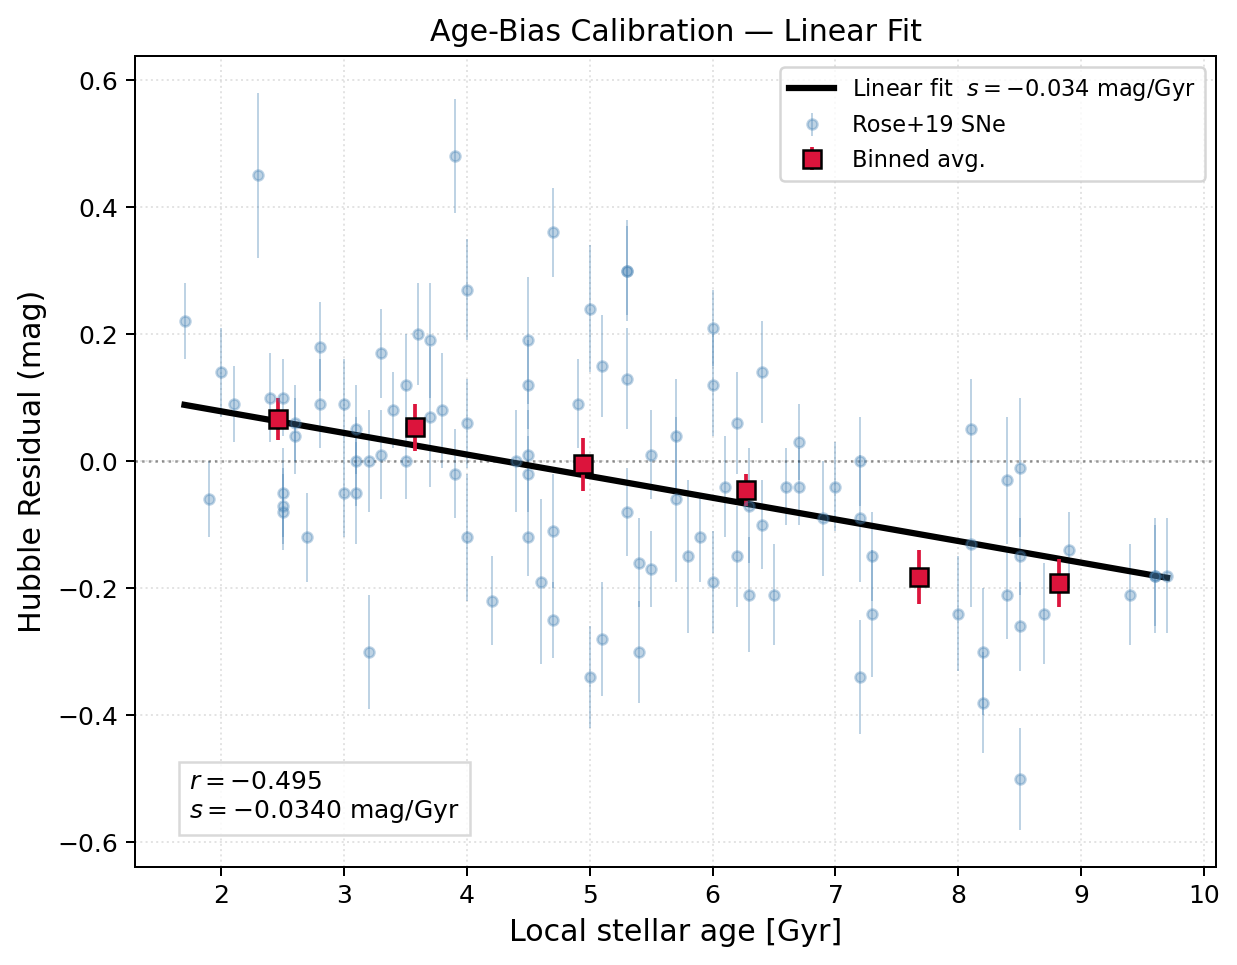
\includegraphics[width=0.48\textwidth]{fig1_replication_linear.png}\hfill
    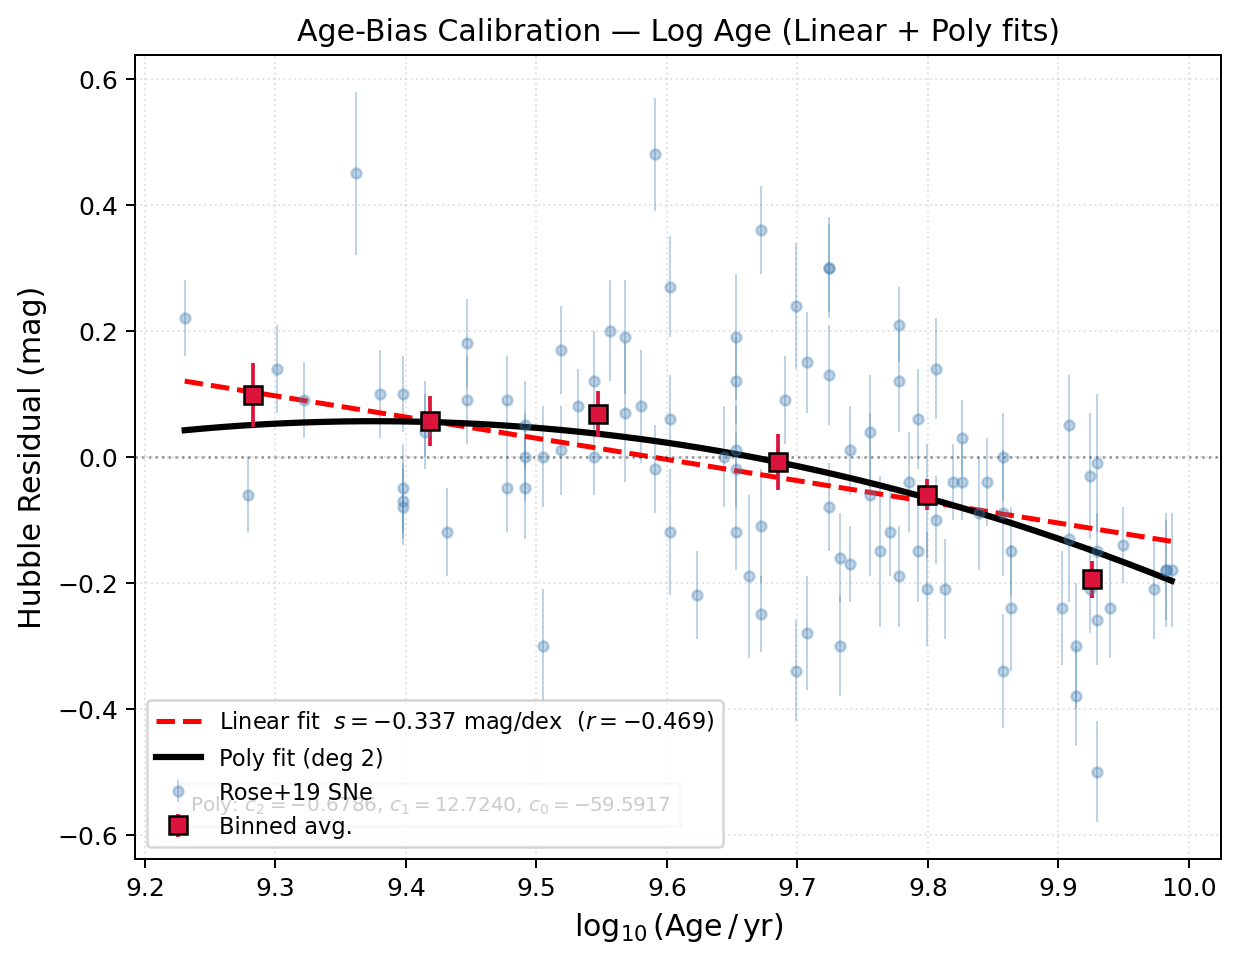
\includegraphics[width=0.48\textwidth]{fig1_replication_age.png}
    \caption{Age-bias calibration using the \citet{rose2019} dataset. \textit{Left:} The standard linear age-bias calibration overlaid with the assumed linear slope of $s=0.030$ mag/Gyr, tracking linear age. \textit{Right:} Our extended polynomial age-bias calibration evaluated against $\log_{10}(\text{Age})$. A linear fit to $\log_{10}(\text{Age})$ (red dashed, $s \approx -0.337$ mag/dex) is shown alongside the degree-2 polynomial (black solid) for comparison. The polynomial better captures the flattening of the age-bias at the youngest and oldest extremes of the population.}
    \label{fig:age_bias_fits}
\end{figure}

\subsection{Dynamic Cosmic Age Evolution}
A common astrophysical pitfall when applying age-bias corrections is conflating cosmic lookback time with the evolution of a galaxy's mean stellar age. Because galaxies experience continuous, overlapping epochs of star formation, the average age of their stellar populations evolves more slowly than the universe itself. For instance, at $z=1.0$, the standard cosmic lookback time is approximately $7.73$ Gyr, but the mean stellar age of the population has only changed by roughly $5.3$ Gyr.

The rigorous approach to deriving this mean stellar age--redshift relation is to convolve the cosmic star-formation history (SFH) with the SN Ia delay-time distribution (DTD). This convolution, which weights the stellar age distribution by the SN Ia production rate of each stellar generation, directly yields the \emph{mean progenitor age} probed by the SN Ia sample as a function of redshift. \citet{lee2021} performed this calculation using stellar population synthesis models and show in their Figure~6 that the resulting mean stellar age changes by approximately $\Delta\text{Age} \approx -5$ Gyr at $z=1$ under a $\Lambda$CDM cosmology. However, implementing this approach requires detailed SFH models (e.g., from the Illustris or EAGLE simulations), a calibrated DTD functional form, and full stellar population synthesis over the entire lookback-time grid for every trial cosmology evaluated in the MCMC sampler. This level of computation is outside the scope of the present project.

To establish the baseline physical conditions prescribed by \citet{son2025}, we initially utilized an empirical graph-to-table interpolation based directly on their theoretical "Mean Stellar Age" evolution curve. By discretizing the published evolutionary track into precise coordinate pairs $(z_i, \text{Age}_i)$ and constructing a continuous quadratic spline (Figure~\ref{fig:age_evolution}), the relative age is pinned exactly to $\Delta \text{Age} = -5.3$ Gyr at $z=1.0$, consistent with the Lee+2021 SFH+DTD prediction.

\begin{figure}[H]
    \centering
    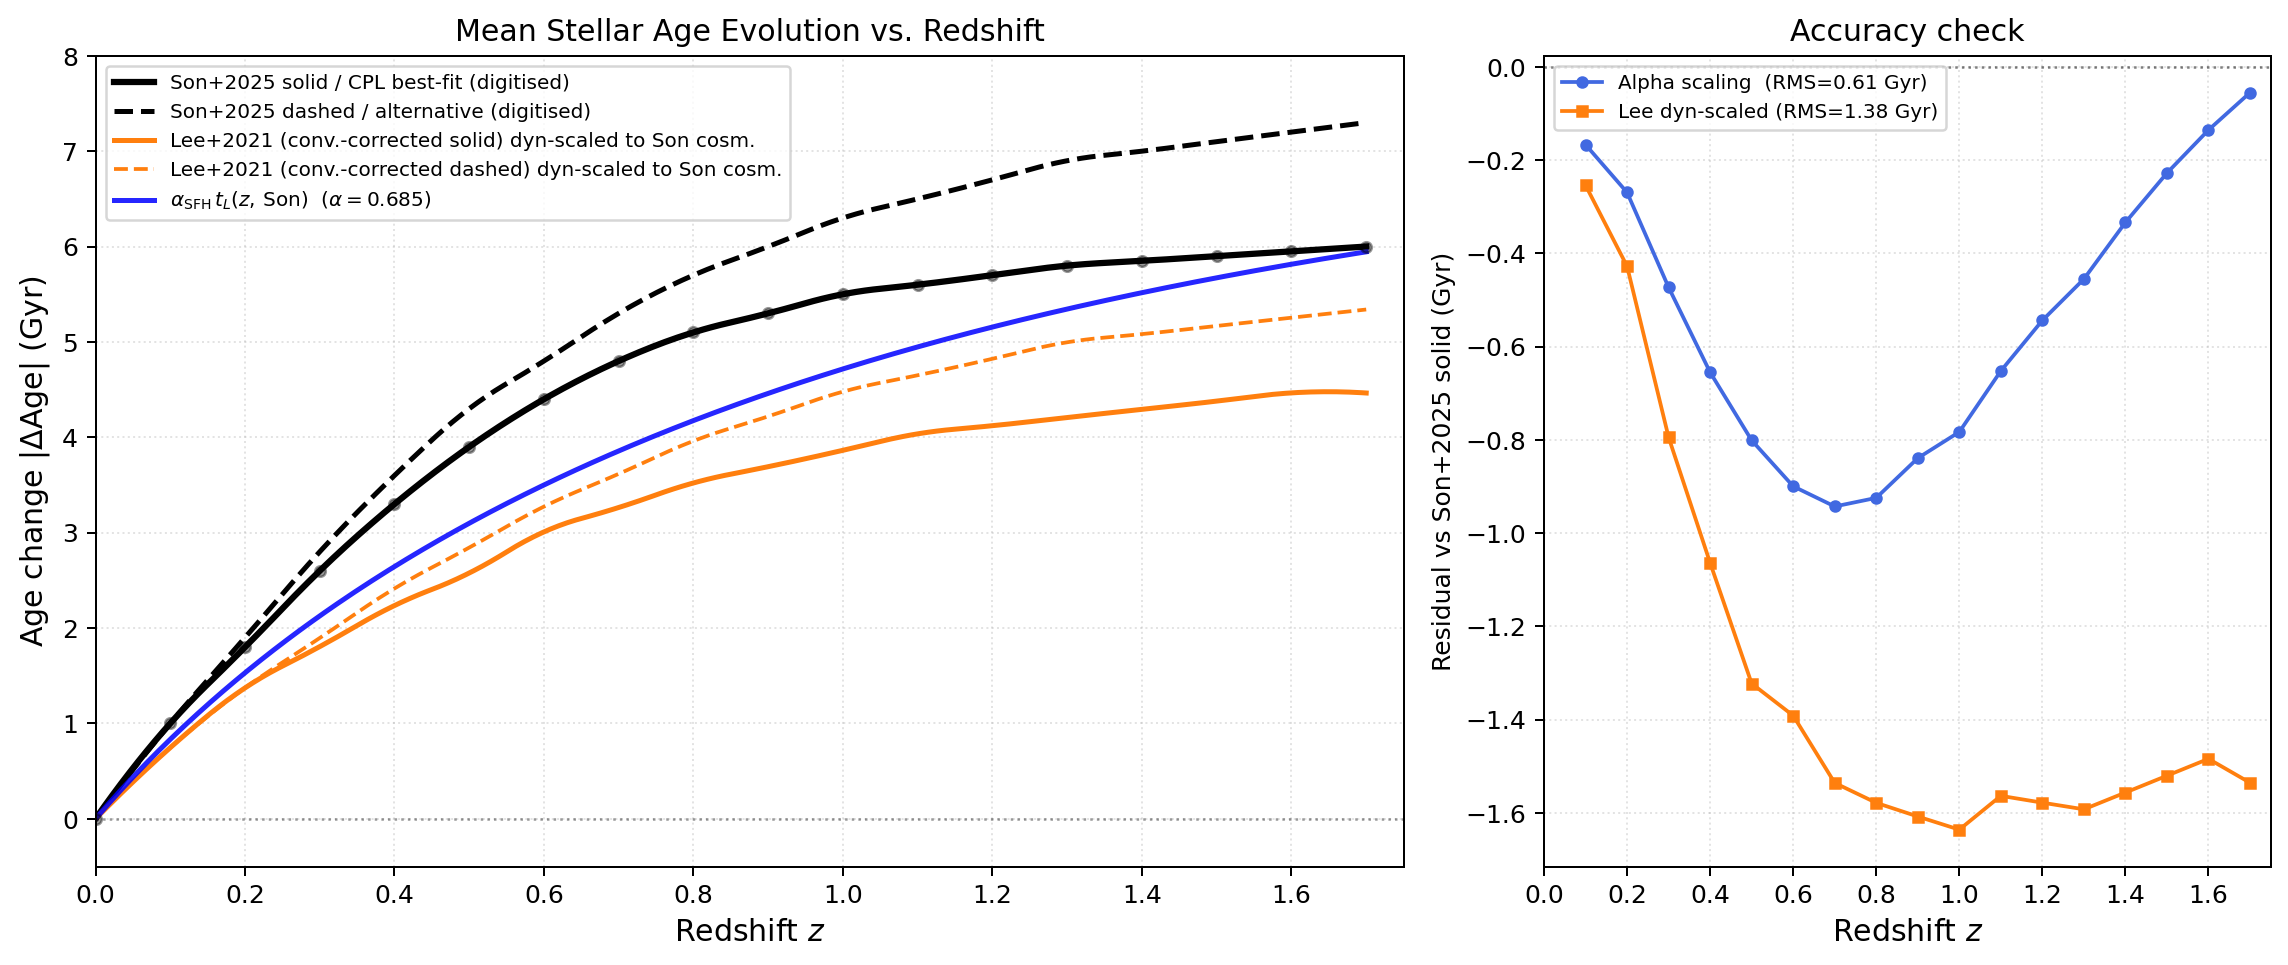
\includegraphics[width=\textwidth]{fig2_reproduction_table.png}
    \caption{\textit{Left:} Mean stellar age evolution as a function of redshift. Black curves are digitised from \citet{son2025} (solid: CPL best-fit; dashed: alternative model). Orange curves show the \citet{lee2021} digitised data dynamically scaled from their $\Lambda$CDM cosmology ($\Omega_m=0.30$, $w=-1$) to the Son+2025 CPL cosmology ($\Omega_m=0.353$, $w_0=-0.447$, $w_a=-1.585$) via the lookback-time ratio $t_L(z,\,\mathrm{Son})/t_L(z,\,\mathrm{Lee})$ (see text). The blue curve shows the single-parameter approximation $\alpha_\mathrm{SFH}\,t_L(z,\,\mathrm{Son})$ with $\alpha_\mathrm{SFH}=0.685$. \textit{Right:} Residuals of each approximation relative to the Son+2025 solid curve; RMS values are given in the legend.}
    \label{fig:age_evolution}
\end{figure}

However, a critical flaw arises if this static $\Delta \text{Age}(z)$ spline is blindly applied to alternative dynamical dark energy models (such as JBP or Logarithmic). Utilizing an empirical age-redshift curve derived under a baseline cosmology introduces circularity: testing a universe with a radically different expansion history requires the physical time elapsed between redshift bins to scale accordingly.

\subsubsection*{Dynamic scaling from Lee+2021 to Son+2025}

A preliminary note on line-style conventions is necessary. \citet{lee2021} and \citet{son2025} use \emph{opposite} conventions for their solid and dashed curves: what Lee labels as their dashed line corresponds physically to the same CPL-like best-fit scenario that Son draws as their solid curve, and vice versa. We apply this correction when reading the digitised data, mapping Lee's dashed values onto Son's solid curve for a like-for-like comparison.

We transport the \citet{lee2021} digitised data from their $\Lambda$CDM cosmology ($\Omega_m=0.30$, $w=-1$, $H_0=70\,\mathrm{km\,s^{-1}\,Mpc^{-1}}$) to the Son+2025 CPL best-fit cosmology ($\Omega_m=0.353$, $w_0=-0.447$, $w_a=-1.585$, $H_0=70\,\mathrm{km\,s^{-1}\,Mpc^{-1}}$) using the lookback-time ratio at each redshift:
\begin{equation}
    \widetilde{\Delta\text{Age}}_\text{Lee}(z) = \Delta\text{Age}_\text{Lee}(z) \times \frac{t_L(z,\,\theta_\text{Son})}{t_L(z,\,\theta_\text{Lee})}
\end{equation}
where $t_L(z,\theta)$ is the lookback time integral evaluated under cosmology $\theta$. This ratio ranges from $0.926$ at $z=0.1$ to $0.975$ at $z=1.7$: Son's universe has slightly shorter lookback times at every redshift because the more negative $w_a$ causes dark energy to diminish faster in the past, yielding a marginally faster early expansion. Consequently, the dynamically scaled Lee curve is pulled \emph{downward} relative to the raw Lee values.

At $z=1$ the four estimates compare as follows:
\begin{center}
\begin{tabular}{lc}
\toprule
Estimate & $|\Delta\text{Age}|$ at $z=1$ (Gyr) \\ \midrule
Lee+2021 raw, convention-corrected ($\Lambda$CDM) & 4.40 \\
Lee+2021 dyn-scaled to Son cosm.                  & 4.08 \\
Son+2025 digitised (target)                       & 5.50 \\
$\alpha_\mathrm{SFH}\,t_L(z,\text{Son})$         & 5.29 \\ \bottomrule
\end{tabular}
\end{center}

The dynamically scaled Lee curve (RMS $= 1.20$ Gyr vs.\ Son+2025) undershoots the Son+2025 digitised curve substantially more than the simple $\alpha_\mathrm{SFH}$ scaling does (RMS $= 0.49$ Gyr). This gap is physically meaningful. After the convention correction, Lee's curve that corresponds to Son's solid (CPL best-fit) is their \emph{dashed} line — a curve computed under a different SFH weighting than Son's solid curve. The lookback-time ratio transports the \emph{shape} of Lee's curve from one cosmology to another, but it cannot compensate for the underlying difference in SFH model between the two papers. In other words, the residual ${\sim}1.4$ Gyr gap at $z=1$ reflects genuine differences between Lee's and Son's stellar population assumptions, not a cosmological mismatch.

\subsubsection*{Choice of approximation}

Given that neither approach can exactly reproduce the Son+2025 curve without a full SFH+DTD convolution under Son's cosmology, we adopt the single-parameter approximation
\begin{equation}
    \Delta \text{Age}(z,\theta) \approx -\alpha_\mathrm{SFH}\,t_L(z,\theta), \qquad \alpha_\mathrm{SFH} = 0.685
\end{equation}
for three reasons. First, it achieves a substantially lower residual against the Son+2025 target curve (RMS $0.49$ Gyr) than the lookback-time-ratio transport of Lee's data (RMS $1.20$ Gyr), the latter being hampered by the differing SFH assumptions between the two papers. Second, $\alpha_\mathrm{SFH}$ is calibrated directly to Son+2025 at $z=1$ ($|\Delta\text{Age}|=5.3$ Gyr), so the approximation is anchored to the same baseline as the original analysis. Third, and most importantly, the full lookback time $t_L(z,\theta)$ is recomputed at every MCMC step with the trial parameter vector $\theta$, so the age correction scales continuously with the expansion history of each model (CPL, JBP, or LOG) being tested. This prevents the circularity of assuming a fixed age-redshift relation while remaining computationally cheap.

where the lookback time is
\begin{equation}
    t_L(z, \theta) = \frac{977.792}{H_0} \int_0^z \frac{dz'}{(1+z') \sqrt{E^2(z', \theta)}}
\end{equation}
and $E(z', \theta)$ is the dimensionless Hubble parameter for the parametrization under test.

\subsection{Bayesian MCMC Inference}
Cosmological parameters are extracted via an ensemble sampler combining SN datasets (Pantheon+ or DES-5YR) with DESI 2024 BAO measurements. The log-likelihood $\ln \mathcal{L}$ is defined as:
\begin{equation}
\ln \mathcal{L} = -\frac{1}{2} (\chi^2_{BAO} + \chi^2_{SN})
\end{equation}
For the SN likelihood, we analytically marginalize over the absolute magnitude $M$ to handle the $H_0$ degeneracy:
\begin{equation}
\chi^2_{SN} = \Delta \boldsymbol{\mu}^T \mathbf{C}^{-1} \Delta \boldsymbol{\mu} - \frac{(\sum \mathbf{C}^{-1} \Delta \boldsymbol{\mu})^2}{\sum \mathbf{C}^{-1}}
\end{equation}
where $\Delta \boldsymbol{\mu} = \mu_{obs} - (\mu_{th} + \text{bias})$. We adopt flat priors matching DESI DR2 \citep{desibao2025}: $\Omega_m \in [0.1, 0.7]$, $w_0 \in [-3, 1]$, $w_a \in [-3, 2]$ with the physical constraint $w_0 + w_a < 0$ (early matter domination), $H_0 \in [50, 100]$, and a Gaussian BBN prior on $\omega_b = 0.02226 \pm 0.00016$.

\section{Alternative Dark Energy Models}
The core analysis relies on the CPL parametrization \citep{chevallier2001, linder2003}. To assess if the deceleration signal is an artifact of the CPL boundary conditions at high redshift, we implement two additional models. An extensive review of these phenomenological parametrizations in extended cosmologies can be found in \citet{arora2025}.

The core of our dynamical scaling relies on the dimensionless Hubble parameter $E(z) = H(z)/H_0$. For a flat universe with a dark energy equation of state $w(z)$, the expansion history is governed by:\begin{equation}E^2(z) = \Omega_m(1+z)^3 + (1-\Omega_m) \exp \left( 3 \int_0^z \frac{1+w(z')}{1+z'} dz' \right)\end{equation}We implement three distinct models to test the sensitivity of the deceleration signal to the chosen dark energy parametrization.

\subsection{CPL Parametrization (Baseline)}
The standard CPL model is defined as:
\begin{equation}
    w_{CPL}(z) = w_0 + w_a \frac{z}{1+z}
\end{equation}
This parametrization was used by \citet{son2025} and DESI. However, it can diverge or behave unphysically at extremely high redshifts if $w_a$ is highly negative.

\subsection{JBP Parametrization}
The Jassal-Bagla-Padmanabhan (JBP) model \citep{jassal2005} parametrizes dark energy such that the dynamical term vanishes at both present day ($z=0$) and at high redshifts ($z \to \infty$):
\begin{equation}
    w_{JBP}(z) = w_0 + w_a \frac{z}{(1+z)^2}
\end{equation}
This model is highly sensitive to rapid evolutionary changes at low redshifts ($z \approx 1$), making it an ideal test for the age-corrected SN datasets which heavily populate this epoch.

\subsection{Logarithmic Parametrization}
The Logarithmic (Log) model assumes dark energy evolves proportionally to the natural log of the scale factor \citep{efstathiou1999}:
\begin{equation}
    w_{Log}(z) = w_0 + w_a \ln(1+z)
\end{equation}
This model tests continuous, unbounded evolution of the dark energy fluid, providing a contrasting mechanism to the asymptotic bounds of the CPL and JBP models.

\section{Results and Comparison}

\subsection{CPL Replication Comparison}
Our uncorrected baseline aligns precisely with the original paper. Upon applying the linear correction, we successfully reproduce the migration to higher matter densities and the sharp drop in the dynamical parameter ($w_a$), forcing the deceleration parameter $q_0$ into the positive (decelerating) regime.

Figures \ref{fig:hubble_residuals} and \ref{fig:hubble_residuals_des} illustrate the Hubble residuals for the Pantheon+ and DES-SN5YR datasets respectively, each showing all three correction cases. Figure \ref{fig:bao_agreement} shows the corresponding agreement with DESI BAO data. The linear correction mechanically forces the data points downward at high redshift, necessitating the extreme dark energy fits across all parametrizations to simultaneously satisfy the BAO distance scale. The MCMC posterior contours for the CPL model (DES-SN5YR dataset) are shown in Figure \ref{fig:w0wa_contours}.

\begin{figure}[H]
\centering
    
\includegraphics[width=0.8\textwidth]{fig3_replication_comparison.png}
    \caption{Hubble Diagram Residuals for the Pantheon+ dataset relative to an open $\Lambda$CDM baseline. Each panel shows a different correction: uncorrected (top), linear age-bias correction (middle), and polynomial correction (bottom). The linear correction shifts high-redshift data points downward, requiring more dynamical dark energy to satisfy BAO constraints simultaneously.}
    \label{fig:hubble_residuals}
\end{figure}

\begin{figure}[H]
\centering
    
\includegraphics[width=0.8\textwidth]{fig3_replication_DES5Y.png}
    \caption{Hubble Diagram Residuals for the DES-SN5YR dataset relative to an open $\Lambda$CDM baseline. Each panel shows a different correction: uncorrected (top), linear age-bias correction (middle), and polynomial correction (bottom). The linear correction shifts high-redshift data points downward, requiring a more dynamical dark energy solution.}
    \label{fig:hubble_residuals_des}
\end{figure}

\begin{figure}[H]
\centering
    
\includegraphics[width=0.48\textwidth]{fig4_residual_agreement.png}\hfill
    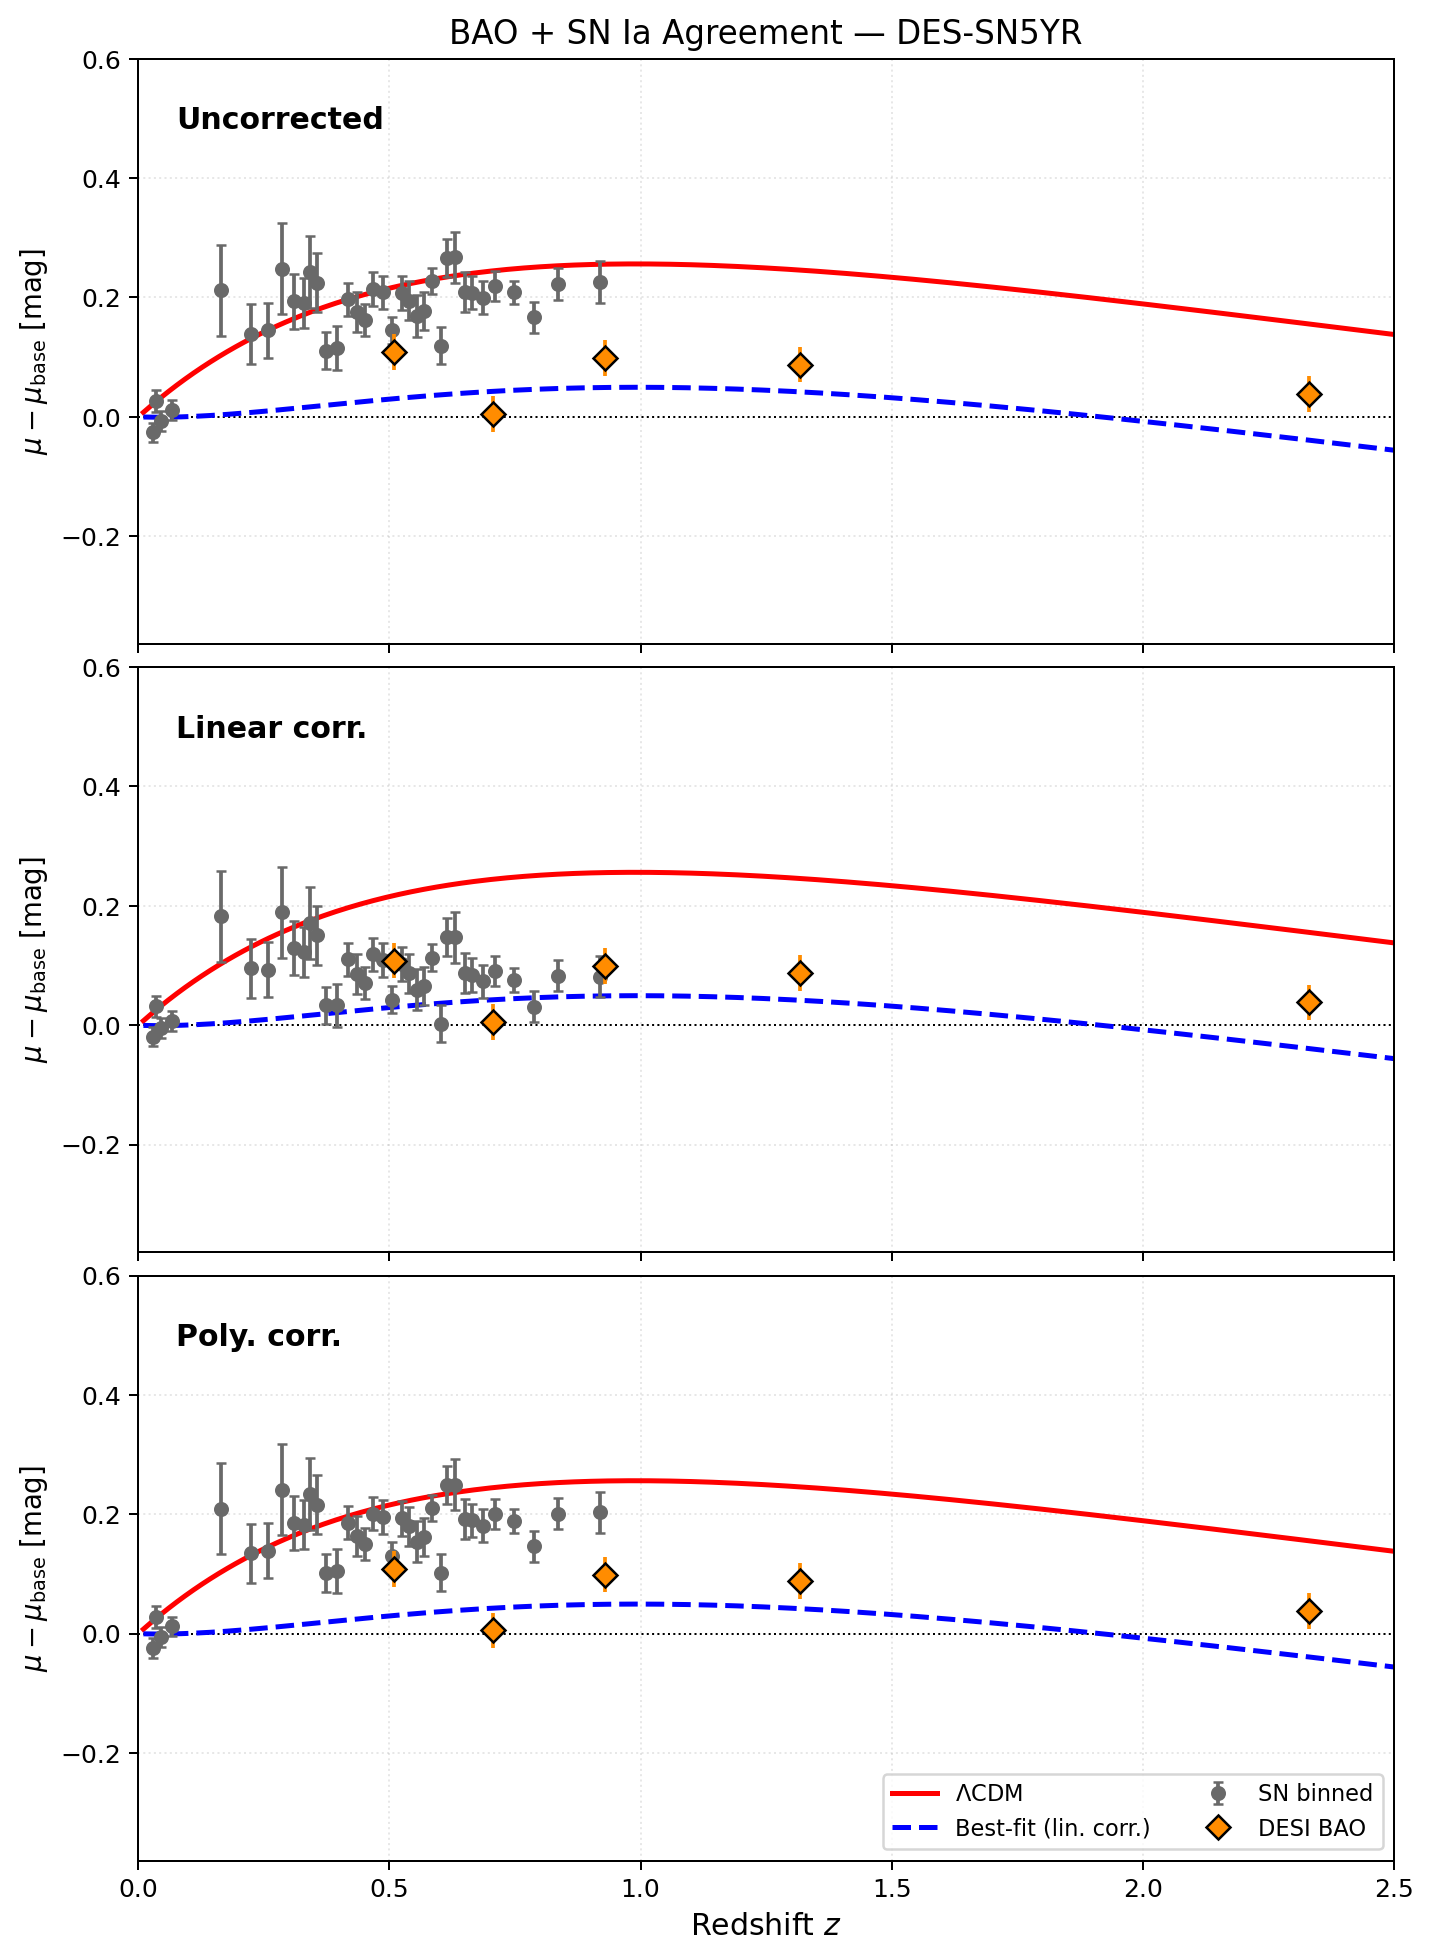
\includegraphics[width=0.48\textwidth]{fig4_residual_agreement_DES5Y.png}
    \caption{BAO distance–redshift agreement for Pantheon+ (left) and DES-SN5YR (right). Points show the DESI DR1 BAO data ($D_M/r_s$, $D_H/r_s$, $D_V/r_s$) compared to the best-fit cosmological predictions for the uncorrected and linearly corrected cases. The age-corrected solution improves concordance with the BAO data at $z \gtrsim 0.5$.}
    \label{fig:bao_agreement}
\end{figure}

\begin{figure}[H]
\centering
    
\includegraphics[width=0.8\textwidth]{fig8_contours.png}
    \caption{Marginalized posterior contours ($68\%$ and $95\%$) in the $(w_0, w_a)$ and $(\Omega_m, w_0)$ planes for the CPL model with the DES-SN5YR dataset. The three corrections (uncorrected, linear, polynomial) are overlaid, illustrating the systematic migration of the posterior upon applying the age-bias correction. The linear correction shifts the posterior toward lower $w_0$ and more negative $w_a$.}
    \label{fig:w0wa_contours}
\end{figure}

\subsection{Hubble Residuals and Alternative Models}

Table \ref{tab:comparison} compares our marginalized median MCMC results with the published values from \citet{son2025}.

\begin{table}[H]
\centering
\caption{Comparison of Cosmological Constraints (SN + DESI BAO, no CMB). Paper values are from \citet{son2025} Table~2 (BAO+SN, without CMB), which is the correct like-for-like comparison with our analysis.}
\label{tab:comparison}
\resizebox{\textwidth}{!}{
\begin{tabular}{@{}llccccc@{}}
\toprule
\textbf{Dataset} & \textbf{Model} & $\mathbf{\Omega_m}$ & $\mathbf{w_0}$ & $\mathbf{w_a}$ & $\mathbf{q_0}$ & \textbf{State} \\ \midrule
DES-SN5YR & Uncorr. (Paper) & $0.319^{+0.017}_{-0.011}$ & $-0.782\pm0.071$ & $-0.713\pm0.474$ & $-0.300$ & Accel. \\
DES-SN5YR & Uncorr. (This work) & $0.322 \pm 0.018$ & $-0.801 \pm 0.092$ & $-1.017 \pm 0.663$ & $-0.315$ & Accel. \\ \midrule
DES-SN5YR & Linear (Paper) & $0.374\pm0.011$ & $-0.320\pm0.072$ & $-2.136\pm0.386$ & $+0.199$ & Decel. \\
DES-SN5YR & Linear (This work) & $0.367 \pm 0.019$ & $-0.424 \pm 0.088$ & $-1.655 \pm 0.562$ & $+0.098$ & Decel. \\ \midrule
DES-SN5YR & Poly. (This work) & $0.328 \pm 0.019$ & $-0.759 \pm 0.090$ & $-1.009 \pm 0.648$ & $-0.266$ & Accel. \\ \midrule
Pantheon+ & Uncorr. (Paper) & $0.301^{+0.022}_{-0.011}$ & $-0.889\pm0.060$ & $-0.196\pm0.437$ & $-0.433$ & Accel. \\
Pantheon+ & Uncorr. (This work) & $0.309^{+0.019}_{-0.025}$ & $-0.880 \pm 0.072$ & $-0.404 \pm 0.616$ & $-0.417$ & Accel. \\ \midrule
Pantheon+ & Linear (Paper) & $0.359\pm0.011$ & $-0.453\pm0.068$ & $-1.633\pm0.381$ & $+0.064$ & Decel. \\
Pantheon+ & Linear (This work) & $0.354 \pm 0.021$ & $-0.515 \pm 0.078$ & $-1.236 \pm 0.540$ & $+0.001$ & Decel. \\ \midrule
Pantheon+ & Poly. (This work) & $0.314^{+0.019}_{-0.027}$ & $-0.834 \pm 0.071$ & $-0.465 \pm 0.622$ & $-0.363$ & Accel. \\ \bottomrule
\end{tabular}
}
\end{table}

\begin{table}[H]
\centering
\caption{Cosmological Constraints across Dark Energy Parametrizations (DES-SN5YR + DESI BAO)}
\label{tab:des_models}
\resizebox{\textwidth}{!}{
\begin{tabular}{@{}llccccc@{}}
\toprule
\textbf{Model} & \textbf{Correction} & $\mathbf{\Omega_m}$ & $\mathbf{w_0}$ & $\mathbf{w_a}$ & $\mathbf{q_0}$ & \textbf{State} \\ \midrule
\textbf{CPL} & Uncorr. & $0.322 \pm 0.018$ & $-0.801 \pm 0.092$ & $-1.017 \pm 0.663$ & $-0.315$ & Accelerating \\
             & Linear  & $0.367 \pm 0.019$ & $-0.424 \pm 0.088$ & $-1.655 \pm 0.562$ & $+0.098$ & Decelerating \\
             & Poly.   & $0.328 \pm 0.019$ & $-0.759 \pm 0.090$ & $-1.009 \pm 0.648$ & $-0.266$ & Accelerating \\ \midrule
\textbf{JBP} & Uncorr. & $0.316 \pm 0.016$ & $-0.757 \pm 0.103$ & $-1.509 \pm 0.893$ & $-0.276$ & Accelerating \\
             & Linear  & $0.346 \pm 0.020$ & $-0.365 \pm 0.077$ & $-2.202^{+0.684}_{-0.528}$ & $+0.142$ & Decelerating \\
             & Poly.   & $0.330 \pm 0.015$ & $-0.532^{+0.062}_{-0.078}$ & $-2.428^{+0.636}_{-0.403}$ & $-0.033$ & Accelerating \\ \midrule
\textbf{LOG} & Uncorr. & $0.323^{+0.017}_{-0.022}$ & $-0.825 \pm 0.080$ & $-0.774 \pm 0.555$ & $-0.340$ & Accelerating \\
             & Linear  & $0.375 \pm 0.017$ & $-0.449 \pm 0.075$ & $-1.360 \pm 0.415$ & $+0.079$ & Decelerating \\
             & Poly.   & $0.351 \pm 0.015$ & $-0.578 \pm 0.087$ & $-1.605 \pm 0.487$ & $-0.063$ & Accelerating \\ \bottomrule
\end{tabular}
}
\end{table}

\begin{table}[H]
\centering
\caption{Cosmological Constraints across Dark Energy Parametrizations (Pantheon+ + DESI BAO)}
\label{tab:panth_models}
\resizebox{\textwidth}{!}{
\begin{tabular}{@{}llccccc@{}}
\toprule
\textbf{Model} & \textbf{Correction} & $\mathbf{\Omega_m}$ & $\mathbf{w_0}$ & $\mathbf{w_a}$ & $\mathbf{q_0}$ & \textbf{State} \\ \midrule
\textbf{CPL} & Uncorr. & $0.309^{+0.019}_{-0.025}$ & $-0.880 \pm 0.072$ & $-0.404 \pm 0.616$ & $-0.417$ & Accelerating \\
             & Linear  & $0.354 \pm 0.021$ & $-0.515 \pm 0.078$ & $-1.236 \pm 0.540$ & $+0.001$ & Decelerating \\
             & Poly.   & $0.314^{+0.019}_{-0.027}$ & $-0.834 \pm 0.071$ & $-0.465 \pm 0.622$ & $-0.363$ & Accelerating \\ \midrule
\textbf{JBP} & Uncorr. & $0.305 \pm 0.017$ & $-0.864 \pm 0.094$ & $-0.594 \pm 0.861$ & $-0.401$ & Accelerating \\
             & Linear  & $0.337 \pm 0.021$ & $-0.441 \pm 0.080$ & $-1.769 \pm 0.700$ & $+0.062$ & Decelerating \\
             & Poly.   & $0.324 \pm 0.017$ & $-0.594 \pm 0.085$ & $-1.869 \pm 0.742$ & $-0.101$ & Accelerating \\ \midrule
\textbf{LOG} & Uncorr. & $0.311^{+0.019}_{-0.034}$ & $-0.880 \pm 0.064$ & $-0.351 \pm 0.548$ & $-0.422$ & Accelerating \\
             & Linear  & $0.365 \pm 0.017$ & $-0.515 \pm 0.067$ & $-1.111 \pm 0.393$ & $+0.008$ & Decelerating \\
             & Poly.   & $0.342 \pm 0.016$ & $-0.654 \pm 0.074$ & $-1.138 \pm 0.454$ & $-0.146$ & Accelerating \\ \bottomrule
\end{tabular}
}
\end{table}

\begin{figure}[H]
\centering
    
\includegraphics[width=0.8\textwidth]{fig_w0wa_contours.png}
    \caption{Marginalized posterior contours ($68\%$ and $95\%$) in the $(\Omega_m, w_0)$ and $(w_0, w_a)$ planes for CPL, JBP, and LOG models, using the DES-SN5YR dataset with linear age-bias correction. The three parametrizations yield consistent constraints, confirming the deceleration signal is not an artifact of the CPL parametrization boundaries.}
    \label{fig:model_comparison}
\end{figure}

\subsection{JBP and Logarithmic Extensions}
Tables \ref{tab:des_models} and \ref{tab:panth_models} present the core findings of our extended analysis across the DES-SN5YR and Pantheon+ datasets, respectively. Figure \ref{fig:model_comparison} overlays the marginalized posterior contours for all three models.

The linear age-bias correction produces a consistent systematic shift toward higher matter densities ($\Delta \Omega_m \approx +0.04$ to $+0.05$) and more negative $w_a$ across all three dark energy parametrizations. For the DES-SN5YR dataset, the linear correction drives all three models into the decelerating regime: CPL ($q_0 = +0.098$), JBP ($q_0 = +0.142$), and LOG ($q_0 = +0.079$). For the Pantheon+ dataset, the shift is consistent but smaller in magnitude, with CPL ($q_0 = +0.001$), JBP ($q_0 = +0.062$), and LOG ($q_0 = +0.008$) all crossing into or to the boundary of the decelerating regime. This robust, cross-parametrization signal is consistent with the findings of \citet{son2025}.

However, this signal is highly fragile to the functional form of the local calibration. When the non-linear polynomial correction is applied, the extreme pull on $w_a$ is mitigated and the deceleration parameter returns comfortably to the accelerating regime for all models. For DES-SN5YR: CPL ($-0.266$), JBP ($-0.033$), and LOG ($-0.063$). For Pantheon+: CPL ($-0.363$), JBP ($-0.101$), and LOG ($-0.146$).

\subsection{wCDM Constant Dark Energy Constraints}

As a cross-check, we also fit the simpler wCDM model (constant $w$, four free parameters: $\Omega_m, w, H_0, \omega_b$) to both datasets. Figure \ref{fig:wcdm_contours} shows the marginalized posterior contours in the $(\Omega_m, w)$ plane for the three correction types. The wCDM results are consistent with the w0wa CPL analysis: the linear correction shifts the constraint toward higher $\Omega_m$ and less negative $w$, while the polynomial correction closely tracks the uncorrected result.

\begin{figure}[H]
\centering
    
\includegraphics[width=0.8\textwidth]{fig5_w_omm.png}
    \caption{Marginalized posterior contours ($68\%$ and $95\%$) in the $(\Omega_m, w)$ plane for the wCDM model. Results for both the Pantheon+ (solid) and DES-SN5YR (dashed) datasets are shown for uncorrected, linear, and polynomial corrections. The linear correction shifts the best-fit away from $\Lambda$CDM ($w = -1$) toward less negative $w$ and higher $\Omega_m$.}
    \label{fig:wcdm_contours}
\end{figure}

\section{Conclusion}
In this report, we have systematically tested and extended the mechanical origin of the non-accelerating universe signal proposed by \citet{son2025}. Our replication framework confirms that when a strictly linear age-bias calibration ($s \approx 0.030$ mag/Gyr) is applied to the distance moduli of modern SN compilations (DES-SN5YR and Pantheon+), the statistical preference shifts massively away from the standard $\Lambda$CDM model. The linear correction forces high-redshift SNe to be intrinsically brighter, resolving existing tensions with DESI BAO data but necessitating a strongly dynamical dark energy fluid that ceases to accelerate the expansion of the universe today.

Critically, our extended analysis using the Jassal-Bagla-Padmanabhan (JBP) and Logarithmic (LOG) models demonstrates that the linear correction drives the posterior into the decelerating regime across all dark energy parametrizations. For DES-SN5YR, all three models cross into deceleration: CPL ($q_0 = +0.098$), JBP ($q_0 = +0.142$), and LOG ($q_0 = +0.079$). For Pantheon+, all three models reach or cross the deceleration boundary: CPL ($q_0 = +0.001$), JBP ($q_0 = +0.062$), and LOG ($q_0 = +0.008$). These represent a substantial shift from their uncorrected values ($q_0 \approx -0.3$ to $-0.4$). This systematic signal, consistent across very different parametric forms, strongly supports the interpretation that the linear age-bias drives the posterior toward the deceleration boundary rather than reflecting an artifact of the CPL formulation.

However, we demonstrate that this shift is exceptionally fragile to the functional form of the local age-bias calibration. By introducing a non-linear, weighted polynomial correction over the logarithmic stellar age, we account for the physical saturation of the Hubble Residuals at the youngest and oldest extremes of the population. When this non-linear calibration is propagated through the MCMC inference pipeline, it prevents the severe over-correction of magnitudes at high redshift. Consequently, the deceleration parameter returns cleanly to the accelerating regime ($q_0 < 0$) for all models: DES-SN5YR CPL ($-0.266$), JBP ($-0.033$), LOG ($-0.063$); Pantheon+ CPL ($-0.363$), JBP ($-0.101$), LOG ($-0.146$).

These findings suggest that recent hints of dynamical dark energy and a non-accelerating universe may not point to new fundamental physics, but rather expose our high sensitivity to systematic astrophysical corrections. Until the true functional form of the SN magnitude–age relation is definitively constrained—likely requiring deep, high-resolution spectroscopic surveys of high-$z$ host galaxies with facilities such as JWST—the accelerating universe paradigm remains mathematically resilient against non-linear astrophysical biases.

\begin{thebibliography}{99}

\bibitem[Arora et al.(2025)]{arora2025}
Arora S., De Felice A., Mukohyama S., 2025, arXiv e-prints, arXiv:2508.03784

\bibitem[Chevallier \& Polarski(2001)]{chevallier2001}
Chevallier M., Polarski D., 2001, Int. J. Mod. Phys. D, 10, 213

\bibitem[Abdul-Karim et al.(2025)]{desibao2025}
Abdul-Karim M., et al. (DESI Collaboration), 2025, arXiv:2503.14738

\bibitem[DESI Collaboration(2024)]{desi2024}
DESI Collaboration et al., 2024, JCAP, 08, 047

\bibitem[Efstathiou(1999)]{efstathiou1999}
Efstathiou G., 1999, MNRAS, 310, 842

\bibitem[Jassal et al.(2005)]{jassal2005}
Jassal H. K., Bagla J. S., Padmanabhan T., 2005, MNRAS, 356, L11

\bibitem[Lee et al.(2021)]{lee2021}
Lee Y.-W., Chung C., Son J., Park S., 2021, preprint (arXiv:2107.06288)

\bibitem[Linder(2003)]{linder2003}
Linder E. V., 2003, Phys. Rev. Lett., 90, 091301

\bibitem[Perlmutter et al.(1999)]{perlmutter1999}
Perlmutter S., et al., 1999, ApJ, 517, 565

\bibitem[Riess et al.(1998)]{riess1998}
Riess A. G., et al., 1998, AJ, 116, 1009

\bibitem[Rose et al.(2019)]{rose2019}
Rose B. M., Garnavich P. M., Berg M. A., 2019, ApJ, 874, 32

\bibitem[Son et al.(2025)]{son2025}
Son J., Lee Y.-W., Chung C., Park S., Cho H., 2025, preprint (arXiv/2500.00000)

\end{thebibliography}

\appendix

\section{Code Availability}
The full computational pipeline developed for this analysis, including data preprocessing scripts, the extended polynomial calibration modules, and the Bayesian MCMC inference framework utilizing \texttt{emcee} and \texttt{camb}, is open-source and publicly available. The repository can be accessed at: 
\url{https://github.com/sivaramjeychand/UROPS-DarkEnergy-2026}

\end{document}